\blfootnote{Adapted from: Martí‐Juan, G., Sanroma‐Guell, G., Cacciaglia, R., Falcon, C., Operto, G., Molinuevo, J. L., … Piella, G. (2020). Nonlinear interaction between APOE$\varepsilon$ 4 allele load and age in the hippocampal surface of cognitively intact individuals. Human Brain Mapping, hbm.25202. \url{https://doi.org/10.1002/hbm.25202}}

\section{Introduction}
\label{sec:introduction}
Alzheimer's Disease (AD) is a neurodegenerative disorder characterized by a progressive decline in multiple cognitive domains and severe brain atrophy. AD affects millions of elderly people worldwide \cite{AlzheimersAssociation} and despite major research efforts to halt or reverse the degenerative process, it has no cure. The major genetic risk factor for AD is the Apolipoprotein E (APOE) $\varepsilon$4 allele \cite{Saunders1993}. The main function of APOE in the brain is cholesterol transport \cite{Saunders1993}, and it modulates various pathways related to AD pathogenesis, including $A\beta$ clearance and neuroinflammation \cite{Zhao2018}. APOE has three different alleles in humans ($\varepsilon$2, $\varepsilon$3, and $\varepsilon$4), with the latter (APOE $\varepsilon$4) being linked to increased risk of AD and earlier disease onset in a gene dose-dependent manner \cite{Liu2013a}. The investigation of brain imaging phenotypes related to APOE $\varepsilon$4 in cognitively intact individuals provides the opportunity to reveal early pathological changes. \\

The impact of APOE-$\varepsilon$4 allele load in preclinical subjects can be studied using different neuroimaging biomarkers \cite{Chetelat2013}. For example, decreased cerebral metabolism, as well as increased $A\beta$ deposition, have been observed in cognitively unimpaired individuals in association with the number of $\varepsilon4$ alleles \cite{Reiman2005,Reiman2009}. Concerning the impact on brain morphology, Fouquet et al.\ \cite{Fouquet2014} found in their meta-analysis that the results are "rather discrepant", suggesting that the effect of the allele load on brain morphology is subtle, and difficult to detect. Yet, capitalizing on a cognitively healthy at-risk cohort with a high number or $\varepsilon4$-homozygous individuals, a recent study found similar gene-dose effects in grey matter volumes of cognitively healthy participants \cite{Cacciaglia2018}. \\

The hippocampus is one of the earliest structures undergoing neurodegeneration in the initial stages of the Alzheimer's continuum \cite{Pievani2011}, and it has been used for diagnosis and early prediction of AD \cite{Sanroma2017}. Longitudinal studies confirmed that hippocampal atrophy can appear in asymptomatic subjects at risk of familial AD \cite{Fox1996}. It was also shown that APOE $\varepsilon$4 allele load is associated with the hippocampus morphology, even in cognitively healthy subjects. A difference in the volume of the right hippocampus was found between APOE $\varepsilon$4 carriers and non-carriers \cite{ODwyer2012}. This difference in volume was also detected by Lind et al.\ \cite{Lind2006}, who found it more profound in younger carriers (<65), and by Tondelli et al.\ \cite{Tondelli2012}, who reported right hippocampus changes to be predictive of AD. However, other studies claim that the left hippocampus is more predictive and presents the most significant effects \cite{Csernansky2005}. Shi et al.\ \cite{Shi2014} proposed a multivariate shape analysis of the hippocampus, studying the genetic influence of APOE in patients at different stages of AD. They found differences between carriers and non-carriers in the left hippocampus for cognitively normal (CN) and mild cognitive impaired (MCI) patients, and for demented patients. In a more recent work, Dong et al.\ \cite{Dong2019} used the same method as in \cite{Shi2014} on a cohort of cognitively unimpaired subjects. Results found a more pronounced effect on the left hippocampus. Other studies found no remarkable volumetric differences between carriers and non-carriers \cite{Hostage2013,Protas2013}, whereas more recent ones found differences in hippocampal subfields, but only for early-onset AD \cite{Parker2019}. The seemingly contradictory results of those studies show that the effect of APOE $\varepsilon$4 load on healthy brains is still not clear. This could be due to several reasons: the use of different methodologies, the low signal of the effect, which makes it difficult to detect it, or the modulation of the effect by other factors, which could make such effect non-homogeneous across subjects. \\

% Paragraph on age and interaction.
Some studies suggest an interaction between age and APOE $\varepsilon$4 allele load effect \cite{Tuminello2011}, arguing that APOE effect on the brain could depend on the age of the subject. Mueller et al.\ \cite{Mueller2009} found significant differences in hippocampal volume between carriers and non-carriers, and effects of age in different subfields (CA3 and DG) of the hippocampus. In a previous work \cite{Mueller2008}, they had found an effect of APOE $\varepsilon$4 in healthy older subjects, but not in younger. Ten Kate et al.\ \cite{TenKate2016} found an interaction with grey matter volume values, and Cacciaglia et al.\ \cite{Cacciaglia2018} showed significant interactions between APOE homozygotes and age on the volume of the right hippocampus, as well as in other brain structures. \\

%% Paragraph on shape analysis
Previously described interactions are based on volumetric data, so more subtle morphology changes unrelated to volume difference might be missed. Shape analysis complements volumetric analysis and can identify and locate subtle regional abnormalities in brain structures, even if there are no changes in volume. Many different approaches have been proposed to capture and study morphological shape changes in brain structures \cite{Nitzken2014,Zhang2016,Shen2017a}. Surface-based shape representation by using spherical harmonics as a parametric descriptor (SPHARM) \cite{Styner2006}, is a common approach for subcortical regions, including the hippocampus \cite{Shen2003,Styner2004,Shi2007,Zhao2008}, with recent works that also incorporate subfield information to the analysis \cite{Cong2015,Inlow2016}. Another approach is to use the hippocampal radial distance \cite{Thompson2004}, relating surface points to a medial curve of each object \cite{Bouix2005,Morra2009,Apostolova2010,Costafreda2011,Chung2010}. Deformation based representations, where descriptors of the shape are defined by the deformation obtained by registering the image to the desired template \cite{Kim2015a,Joshi2016}, are also frequently used. A popular framework for this approach is the large deformation diffeomorphic metric mapping \cite{Beg2005,Miller2006}, which uses diffeomorphic transformations to parametrize the different shapes and map the template to each subject. Several methods based on this framework have been proposed and applied in subcortical brain structures \cite{Vaillant2007,Durrleman2014,Singh2014,Younes2014,Miller2015,Li2017f}, including the hippocampus \cite{Qiu2009,Tang2016,Cury2018}. Other different methods have been proposed, such as Bayesian-based analysis \cite{Gori2017,Gutierrez2019}, or spectral matching \cite{Shakeri2016a}. Some studies also incorporate longitudinal shape changes into the analysis to capture and analyze shape trajectories along time \cite{Miller2015,Bone2018,Cury2019a}. Recently, software tools allowing for easy shape processing and analysis have been made available, such as ShapeWorks \cite{Cates2017}, implementing a particle-based model without parametrization, or Deformetrica \cite{Bone2018a}, using the large deformation diffeomorphic metric framework for various functionalities. Comparison and validation of such tools and methods show that some performance inconsistencies remain \cite{Madan2017,Gao2014,Goparaju2018}, and research on the field is still expanding. \\

Our objective is to study the effects and interactions of APOE allele load on the hippocampal morphology of cognitively unimpaired subjects at risk of AD. To that end, we analyze linear and non-linear interactions between APOE $\varepsilon$4 allele load and age on the geometric differences on the surfaces of normalized shapes. We present our results on two cohorts: 1) The ALFA cohort \cite{Molinuevo2016}, composed of cognitively healthy participants enriched with individuals at higher genetic risk for AD, and 2) the ADNI cohort \cite{Mueller2005}, containing a mixture of healthy and cognitively impaired subjects with different degrees of AD pathology. The reason for analyzing this second population is twofold. First, to study whether the APOE $\varepsilon$4 effect in the first cohort has some resemblance or affinity to the AD effect in the second cohort; that is, we want to explore if the effect of different APOE allele load is related to the effect produced by the disease on hippocampal shape. And second, to evaluate whether APOE $\varepsilon$4 allele load has a similar effect in both cohorts. We segment the hippocampus and use a diffeomorphic registration approach to generate the corresponding meshes. We use multivariate statistical shape analysis to detect subtle surface changes that could be undetectable when analyzing structural volume or grey matter density. We analyze the effects of multiple factors on hippocampal morphology, namely, APOE, age, sex, and diagnosis (when applicable), study linear and non-linear interactions between age, APOE and diagnosis, and we quantified the similarity between different effects on the two populations. The proposed shape analysis method allows visualizing both the magnitude and the direction of the effect on the whole surface of the hippocampus, thus providing new insights about the corrected effect of APOE $\varepsilon$4 (and other factors) on hippocampal morphology.  \\

\section{Methods}
\label{sec:methods}

In this section, we detail the pipeline of our method to extract the hippocampal meshes from the imaging data and the experimental design. All code to reproduce the pipeline and experiments described here can be found in the repository of the project\footnote{\url{https://github.com/GerardMJuan/hippo-surf-analysis}}.

\subsection{Subjects}

We analyzed two cohorts: \\

1. \textbf{ALzheimer and FAmilies (ALFA)} study \cite{Molinuevo2016}, a genetically enriched dataset of cognitively healthy subjects with a high proportion of $\varepsilon4$. These are pooled between non-carriers (NC), heterozygotes (HE), carrying one copy of the allele, and homozygotes (HO), carrying two copies. This cohort is ideal to study early pathophysiological effects of AD and the possible effects of APOE $\varepsilon$4 in the preclinical phase of the disease. 518 subjects from the cohort were used for this study. Magnetic resonance imaging (MRI) was conducted on a 3T General Electric scanner (GE Discovery MR750 W). Structural 3D high-resolution T1-weighted images were collected using a fast spoiled gradient-echo sequence implementing the following parameters: voxel size = 1 mm$^3$ isotropic, repetition time = 6.16 ms, echo time = 2.33 ms, inversion time = 450 ms, matrix size = $256 \times 256 \times 174$, and flip angle = $12\degree$. \\

2. \textbf{Alzheimer's Disease Neuroimaging Initiative (ADNI)} \cite{Mueller2005}. ADNI is one of the largest longitudinal public datasets on AD, containing not only MRI but also other imaging modalities and genetic information, among others. 1016 subjects from the main study of ADNI were used for this work, to detect affinities between the effect of AD on hippocampus shape and the effect of APOE allele load in cognitively healthy subjects from the ALFA dataset, and to assess the effect of APOE in patients at different stages of the disease. Structural 3D high-resolution T1-weighted MRI scans were available for every subject. ADNI is a multisite study, so there are differences in MRI acquisition between scans. For this reason, in all ADNI tests, we included site as a covariate to correct for possible site differences (Section \ref{subsec:stat}). Further information on image acquisition for the ADNI scans used in this work can be found on \cite{Jack2010a}. \\

\subsection{Pipeline}
\label{sec:pipeline}

Our data processing pipeline consists of four stages: hippocampus segmentation on MRI, image registration to a common template, mesh generation, and shape normalization. Figure \ref{fig:pipeline} shows the full pipeline.

\begin{figure}[htbp]
  \centering
  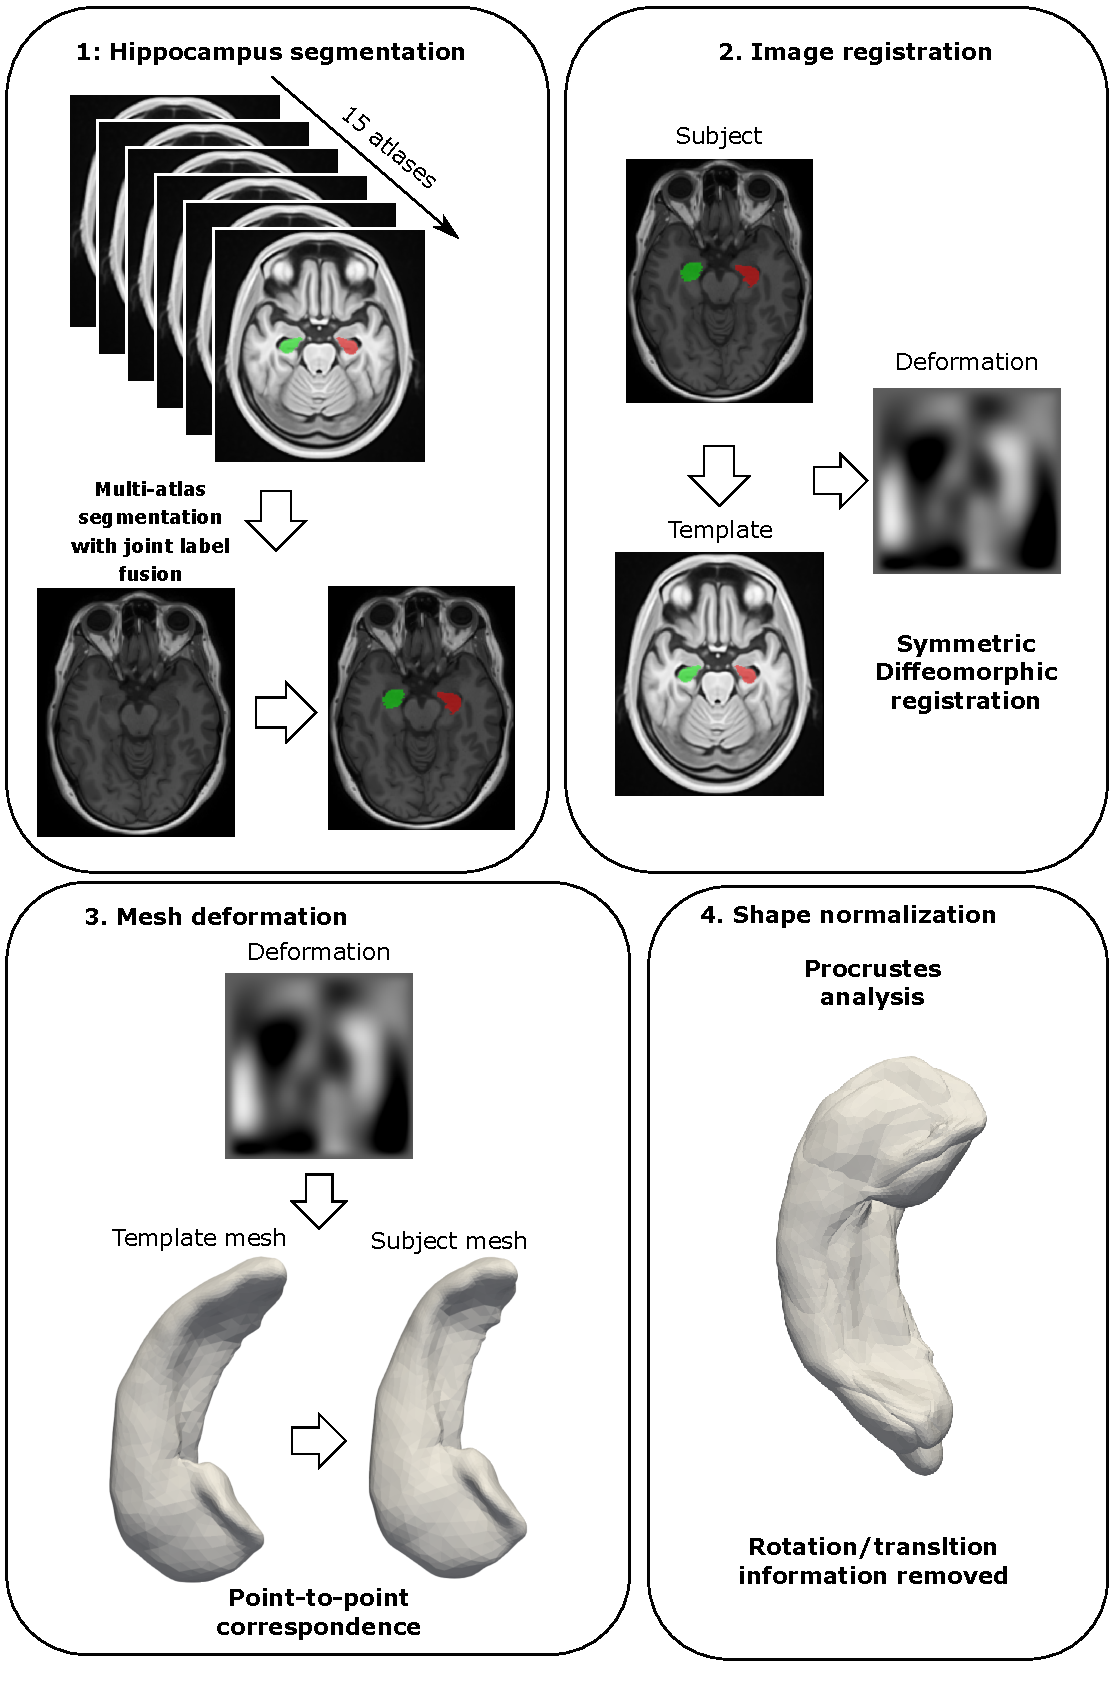
\includegraphics[width=0.9\textwidth]{figures/hippocampus/figure_pipeline.pdf}
  \caption{Outline of the processing pipeline.}\label{fig:pipeline}
\end{figure}

\begin{enumerate}
    \item \textbf{Hippocampus segmentation:} We used a multi-atlas segmentation approach with joint label fusion and corrective learning \cite{Wang2013} to segment the hippocampi. We chose this algorithm, implemented in the ANTs library \cite{Avants2009}, because of its top performance in various segmentation challenges \cite{Wang2013} and good performance when compared to other segmentation methods \cite{Dill2015}. As atlas, we used 15 segmented MRI scans from the ADNI database. The hippocampus segmentation of the atlases, provided by ADNI, were computed using a semi-automatic hippocampal volumetry method \cite{Hsu2002}. The 15 atlases were selected so that they spanned a wide hippocampal shape variability \cite{Sanroma2014}. \\
    
    \item \textbf{Image registration:} We non-rigidly registered each subject's image and its corresponding segmentation to a template image (MNI 152) and its corresponding ground-truth hippocampus segmentation using the symmetric diffeomorphic normalization approach \cite{Avants2008a} implemented in ANTs library. We used two channels, with equal weight, to jointly register the subject image to the template image and the hippocampus segmentation of the subject to the template segmentation. This allowed us to obtain a more precise registration between each image and the template while ensuring that the corresponding segmentations match well. The registration generated a deformation field for each subject. \\
    
    \item \textbf{Mesh deformation:} We used the segmentation from the template image to build a template mesh, using the marching cubes algorithm \cite{Lorensen1987}, giving more vertex density to regions with higher curvature. The deformation fields obtained from the previous registration stage were used to warp the template mesh to each subject space. This procedure ensures that the generated meshes have vertex and triangle correspondences, which directly facilitates the downstream statistical analysis. \\

    \item \textbf{Shape normalization:} After obtaining all the individual meshes, we processed them to remove undesired variation. Since we are interested in shape changes, we aligned the meshes using Procrustes analysis \cite{Gower1975} to compensate rotational and translational variations not already removed in the registration stage. Unlike the normal Procrustes analysis, scaling was not performed to preserve the size information. Even if some meshes present large atrophied and/or missing regions, with the point-to-point correspondence obtained in the previous step they are directly comparable and hence their associated deformations can be captured.
    
\end{enumerate}

We also conducted both automatic and manual quality control to detect segmentation and mesh extraction errors. First, we computed the volumes of each mesh, discarding the meshes that were outliers. Then, we did a manual check of all obtained meshes and discarded those that had obvious visual errors. In total, we removed 39 scans from the original ALFA dataset and 47 scans from ADNI, resulting in 479 and 969 total scans, respectively. Table \ref{table:cohorts} shows the demographic characteristics for both cohorts. \\

\begin{table}[htbp]
\resizebox{1\textwidth}{!}{%
\begin{tabular}{@{}clccccc@{}}
\toprule
 & APOE $\varepsilon$4 & Non-carriers & Heterozygotes & Homozygotes & Total & Statistics \\ \midrule 
\multirow{4}{*}{ALFA} & Number & 234 & 187 & 58 & 479 & - \\  
& Age & $57.88\pm7.55$  & $58.55\pm7.41$ & $53.93\pm6.14$ & $57.66\pm7.46$ & F=5.69, P=0.017 \\
& Education & $13.62\pm3.66$ & $13.81\pm3.48$ & $13.59\pm3.35$ & $13.69\pm3.55$ & F=0.03, P=0.852  \\
& Male/Female & 88/146 & 87/100 & 23/35 & 198/281 & $\chi^2=3.48$, P=0.170  \\ 
& MMSE & $28.96\pm1.14$ & $29.14\pm1.00$ & $29.1\pm1.06$ & $29.05\pm1.08$ &  F=1.78, P=0.183    \\
\midrule
\multirow{10}{*}{ADNI}  & Diagnosis  & CN & MCI & AD & Total & Statistics \\ \midrule 
& Number & 281 & 475 & 213 & 969 & - \\ 
& Non-carriers & 203 & 231 & 70 & 504 & - \\
& Heterozygotes & 71 & 189 & 100 & 360 & - \\
& Homozygotes & 7 & 55 & 43 & 105 & - \\ 
& Age & $75.25\pm5.31$ & $74.13\pm7.52$ & $74.91\pm7.49$ & $74.62\pm6.95$ & F=0.56, P=0.456 \\
& Education & $16.15\pm2.78$ & $15.76\pm2.65$ & $14.84\pm3.14$ & $15.67\pm2.99$ & F=22.97, P<0.001  \\
& Male/Female & 144/137 & 298/177 & 109/104 & 551/418 & $\chi^2=13.11$, P=0.001  \\
& MMSE & $29.05\pm1.07$ & $27.2\pm1.82$ & $23.29\pm2.06$ & $26.88\pm2.67$ &  F=1230, P<0.001    \\
\bottomrule
\end{tabular}}
\caption[Demographics characteristics for the studied cohorts.]{Demographics characteristics for the studied cohorts. Age and education presented as average and standard deviation, in years. CN: Cognitively normal. MCI: Mild cognitive impairment. AD: Alzheimer's disease. MMSE: Mini-mental state examination.}\label{table:cohorts}
\end{table}

\subsection{Statistical analysis}
\label{subsec:stat}

Using the mean mesh (after Procrustes) as a reference mesh, we defined $y_i=(y_{i0}, y_{i1}, y_{i2}) \in \mathbb{R}^3$ as the vector of the residuals between the i-th vertex coordinates of the subject mesh and the reference mesh. The choice of reference is irrelevant for the analysis since the bias term in the regression ensures that the origin corresponds to the population mean for each vertex. \\

The model at each vertex $i$ for each dimension $j$ is a multiple regression model with interaction terms of the form:

\begin{equation}
    y_{ij} = \alpha_{j} + \sum_{k \in \mathcal{\varphi}} \beta_{kj} c_k + \varepsilon_j \textrm{ for } j = {0, 1, 2},
\end{equation} 

where $\alpha$ is the intercept, $\beta_{kj}$ is the coefficient for covariate or interaction $c_k$, $\mathcal{\varphi}$ is the set of indices of covariates and their interactions, and $\varepsilon$ is the error term. Left and right hippocampus were analyzed separately. \\ 

APOE $\varepsilon$4 status was included as a covariate. We considered an additive model as well as dominant and recessive models. For the additive model, the allele variable indicated the number of copies of the $\varepsilon$4 allele (e.g. 0, 1, or 2). For the dominant and recessive models, we used binary (aka dummy) variables. In the dominant model, the variable coded the presence or absence of the $\varepsilon$4 allele (e.g. 0 indicating zero copies of the risk allele and 1 indicating one or two copies). In the recessive model, the variable coded the presence or absence of two copies of the $\varepsilon$4 allele (e.g. 0 corresponding to zero or one copies of the risk allele). \\

The previous models assume that the AD risk of APOE $\varepsilon$4 is linear with the number of alleles, and they do not account for the potentially reduced risk of APOE $\varepsilon$2, which has been well documented \cite{Genin2011,Liu2013a}. For this reason, we also used a model that includes the associated AD risk for each allele pair. AD risk was included from \cite{Reiman2020}, which defined AD risk for different APOE allele pairs in a cohort of over 5000 neuropathologically characterized AD and control participants. We encoded the odds ratio (OR) of AD risk of each allele pair compared to $\varepsilon$3$\varepsilon$3 and applied a logarithm to linearize the risk values and normalize the residuals. Table \ref{table:apoeallele} shows the distribution of allele pairs over both datasets. \\

\begin{table}[htbp]
\centering
\resizebox{0.75\textwidth}{!}{%
\begin{tabular}{@{}cccccccc@{}}
\toprule
      & \multicolumn{3}{c}{Non-carriers} & \multicolumn{2}{c}{HE} & HO   &       \\ 
     & $\varepsilon$2$\varepsilon$2      & $\varepsilon$2$\varepsilon$3      & $\varepsilon$3$\varepsilon$3  &  $\varepsilon$2$\varepsilon$4       & $\varepsilon$3$\varepsilon$4      & $\varepsilon$4$\varepsilon$4 & Total \\ \midrule
ADNI  & 3         & 67        & 434      & 22         & 338       & 105  & 969   \\
ALFA  & 7         & 97        & 130      & 38         & 149       & 58   & 479   \\
Total & 10        & 164       & 564      & 60         & 487       & 163  & 1448  \\ \bottomrule
\end{tabular}}
\caption[APOE allele pair counts.]{APOE allele pair counts for the studied cohorts. HE: heterozygotes. HO: homozygotes.}\label{table:apoeallele}
\end{table}

We also included, as covariates, age, sex, and years of education. In the experiments that included ADNI subjects, we also included diagnosis (DX) and site, a variable that accounts for the different sites where images were captured. Age was centred at its respective mean to limit the effects of multicollinearity when evaluating the quadratic effects. \\

For the statistical analysis, we combined the univariate T statistics over all coordinates into a single statistic, by finding the maximum over all possible linear combinations. This maximum is the Hotelling's T statistic \cite{Hotelling2007}. This final T-statistic was then used to test for significance of the effects. As the number of vertices was large, we corrected for multiple comparisons to remove false positives and obtained significant clusters of vertices over the hippocampal surface. We applied family-wise error correction with random field theory to account for spatial correlation \cite{Hayasaka2004} We selected only significant clusters with a number of vertices larger than a given threshold to further remove false positives. We set that threshold to 20. \\

\subsection{Experimental design}
\label{subsec:exp}

We defined three different settings for our experiments, depending on the data used. Alignment of the meshes before analysis, as described in Section \ref{sec:pipeline}, was done independently for each of the settings. For each setting, we analyzed a model with no interaction terms (we refer to this model as the base model), and several models with the specified interaction terms. Each model was evaluated using the different APOE encodings previously mentioned:

\begin{itemize}
    \item Case I: the analysis was performed on the ALFA cohort. We added to the base model the interaction terms between age (linear and squared) and APOE. 
    \item Case II: the analysis was performed on the ADNI cohort. We added to the base model the diagnosis information and interaction terms between age (linear and squared) and APOE, age and diagnosis, and diagnosis and APOE.
    \item Case III: the analysis was performed on the healthy subjects of the ADNI cohort. Despite the low amount of samples and the small proportion of homozygotes, we wanted to test for interactions between age (linear and squared) and APOE to see if the effect of the interactions could be compared to the effect obtained in the ALFA experiments.
\end{itemize}

We also considered a fourth setting, which jointly analyzed both cohorts, considering ALFA subjects to be a new site and having CN as the diagnosis. We repeated all previous tests for this joint dataset. However, the results were not included in the main text as no significant regions were observed; they can be found in Supplementary Table S1 (base model) and S2 (interaction model between APOE and age). All the models and experiments were implemented in MATLAB using the SurfStat toolbox \cite{Worsley2009}.\\ 

\subsection{Visualization and effect comparison}
\label{sec:visualization}

For better visualization of the effect of each factor and interaction over the hippocampal surface, we defined a 3D vector for each vertex $i$ and effect $k \in \mathcal{\varphi}$: $b^k_{i} = (\beta_{k0}, \beta_{k1}, \beta_{k2}). $ Note that this vector does not represent deformation, but rather the effect of the indicated factor on that vertex (i.e. points of the surface). We defined the colour of the effect depending on whether it is a contraction (dark violet, negative values) or expansion (light yellow, positive values) displacement, with respect to the normal of the template surface at that mesh point, and the strength of the effect. Note that, given these criteria, some artefacts could appear in the colouration depending on whether the effect is close to being orthogonal to the normal. In the representation shown in the figures, arrow length and size indicate a stronger effect. The arrows are distributed equally over the vertices for easier visualization.  \\

To quantitatively compare and quantify the similarity between the results of two different effect maps, we used cosine similarity. For two vector effects $b1$ and $b2$ located on the same vertex $i$,  but coming from different experiments:

\begin{equation}
S(b1, b2) = \frac{b1\cdot b2}{\|b1\|\|b2\|}.
\end{equation}

This metric was selected for effect comparison because it allows us to highlight and quantify the similarity of the effect direction over the surface. We do not want to compare the strength of the effect, which, given the differences between cohorts, could greatly vary and be misleading. The cosine similarity was rescaled to lie between 0 (i.e. vectors have opposite directions) and 1 (i.e. vectors have the same direction), with 0.5 indicating orthogonality between the two vectors. \\

To test the statistical significance of the similarity, we performed a randomisation test, which corrects for multiple comparisons. We first created a distribution of similarities for a large number K of pairs of random vectors $k = (k_0, k_1, k_2)$, with $k \sim \mathcal{N}(0,\,1)^3$. We set $K=100000$. Then, we assessed, for each similarity value, its percentile over the distribution, obtaining the corresponding p-value. Finally, we selected clusters of vertices with p<0.05, removing those with less than 20 vertices to further reduce false positives. In this way, we can detect relevant local areas where there is a strong similarity. \\

We compared the similarity of the effects obtained between ALFA and ADNI base models, ALFA interaction and ADNI base models, and ALFA and ADNI interaction models. We also wanted to assess if detected APOE effects and interactions in ALFA were similar to those in ADNI. For this reason, we compared the similarity between ALFA and healthy patients in ADNI base and interaction models, and ALFA and ALFA plus ADNI, base and interaction models.

\section{Results}
\label{sec:results}

\subsection{ALFA dataset}

Table \ref{table:fullALFAtable} summarizes the main results for all experiments done on the ALFA cohort. Results are shown for the base model, a model with a linear interaction term between APOE and age, and another with a linear and squared interaction. The "Results" column shows the general statistical results, whereas the "Cluster analysis" column shows information about the detected clusters on the hippocampal surface after correction. More than one line for a single test shows that more than one significant cluster was detected for that test. \\

\begin{table}[htbp]
\centering
\resizebox{0.9\textwidth}{!}{%
\begin{tabular}{@{}c|c||ccc||ccc@{}}
\toprule
 & \multirow{2}{*}{Test} & \multicolumn{3}{c||}{Results}  & \multicolumn{3}{c}{Cluster analysis} \\  \cline{3-5} \cline{6-8}
 &  & Hipp & Avg. T & Max. T & N & $P_{peak}$ & $P_{cluster}$ \\ \midrule
\multirow{15}{*}{\rotatebox[origin=c]{90}{Base model}} & Age &    R &   1.34 & 9.64 &  2121  &    <$.001$ &   <$.001$\\
 &  &    L &   1.24 &   8.41 & 1898 &     <$.001$ &   <$.001$ \\ 
& Sex &    R &   2.23 &  12.17 &  2605 &    <$.001$  &  <$.001$\\
&  &  L &   2.28 &  13.15 &  2438 &    <$.001$ &   <$.001$ \\
& Years ed. &    R &   0.58 &   2.75 &  - &   -  &  - \\
&  &  L &     0.61 &   3.04 &  - &  - &  - \\
 & APOE (Additive) &    R &   0.55 &    2.4 & - &  - & - \\
 &  &  L &   0.63 &    3.1 &  - &  - & - \\
 & APOE (Dominant) &  R &   0.56 &   2.38 & - & - & - \\
&   &   L &   0.64 &   3.12 &   - &  - & - \\
 & APOE (Recessive) &   R &   0.61 &   2.61  &  - & - & - \\
&  &    L &   0.63 &   2.89 & - &  - & - \\ 
 & APOE ($\log$(OR)) & R  &  0.58 &   2.62 & - & - & - \\
&  & L & 0.61 &  2.96 & - & -  & - \\ \midrule
 \multirow{8}{*}{\rotatebox[origin=c]{90}{\hspace{1pt} Linear int. model \hspace{1pt}}} & APOE (Add)$\times$Age &    R &   0.68 &    4.02 &    50 &    0.093 &   0.012\rule{0pt}{2.6ex} \\
&                       &    L &   0.68 &   4.12 &  172 &    0.068 &     0.006 \\
& APOE (Dom)$\times$Age &    R &   0.69 &   4.09 &    48 &    0.079 &     0.016 \\
&                       &    L &   0.67 &   3.88 &  135 &  0.141 &     0.015\\
& APOE (HO>NC)$\times$Age &    R &   0.72 &   4.16 &    50 &    0.06 &      0.02 \\
 &                       &    L &   0.68 &   4.30 &  150 &   0.038 &     0.005 \\ 
 &APOE ($\log$(OR))$\times$Age &    R &  0.69 &   3.67 & - & - & -  \\
 &                       &    L &  0.67 &   4.08 & -  & - & -  \\ \midrule 
 \multirow{11}{*}{\rotatebox[origin=c]{90}{Squared int. model}} & APOE (Add)$\times$Age &  R &   0.85 &   4.57 &  260 &   0.015 &     0.001 \\
 &                       &   L &    0.7 &   3.17 &   - & - & - \\
& APOE (Add)$\times$Age$^2$ &   R &   0.78 &   4.67  &  270 &   0.01 &   <$.001$ \\
&                          &    L &   0.65 &   3.14 &  - & - & - \\
& APOE (HE > NC)$\times$Age &    R &   0.92 &   4.23 &    313 &    0.045 &     0.004 \\
&                      &    L &   0.78 &   3.19 & - &  - & - \\
& APOE (HE > NC)$\times$Age$^2$ &   R &   0.82 &   4.31 &  333 &    0.037 &     0.002 \\
&                               &   L &    0.7 &   3.18 & - &  - & - \\
& APOE ($\log$(OR))$\times$Age$^2$ &   R & 0.81 &   4.69 & 86 & 0.009 &  0.003 \\
&                                  &     &     &         &  44 & 0.012 & 0.004 \\
&                                  &   L &   0.66 &   3.24 & - & - & - \\ \bottomrule
\end{tabular}}
\caption[Results obtained on the ALFA cohort for base, linear interaction, and squared interaction models.]{\small Results obtained on the ALFA cohort for base, linear interaction, and squared interaction models. General test results and information about significant clusters that survived correction are included. Results are divided by model (base, linear interaction or squared interaction). Hipp indicates left (L) or right (R) hippocampus. Max. and Avg. T are the maximum and average Hotelling's T statistic over all vertices, respectively. XX > YY indicates the comparison used for that specific test. For the cluster analysis after correction, N is the number of vertices of the significant cluster. $P_{peak}$ and $P_{cluster}$ are the random field corrected p-values for the peak point and the whole cluster, respectively. Only clusters with N > 20 and $P_{cluster} < 0.05$ are included. Rec: recessive. Add: additive. Dom: dominant. OR: Odds ratio of AD risk.}\label{table:fullALFAtable}
\end{table}

For the base model, Table \ref{table:fullALFAtable} (upper part) summarizes the effect of each covariate (age, sex, years of education and APOE) over the mesh for the base model without interactions, and its detected significant clusters. No significant clusters were found for any of the APOE contrasts. Figure \ref{fig:alfabaselinefig1} shows the effect of selected covariates over the hippocampus mesh. We can observe strong effects for age, with a large association with surface expansion at zones on the head and tail of the hippocampus, and contraction in the body; and sex, with a general contraction effect that is largely associated to intra-cranial volume (as we did not correct for it in the preprocessing to not remove relevant information). For the linear interaction model, \ref{table:fullALFAtable} (middle part) summarizes the effects in the model with a linear interaction between APOE and age, focusing on additive, dominant, and APOE OR effects, and the differences between homozygotes and non-carriers. Corresponding significant clusters are also included. For the effects of the APOE and age interaction between HO and NC groups, a significant cluster associated with a linear expansion effect was detected in the head of both hippocampi. Supplementary Figures S3 and S4 show the effects of the APOE and age interaction, between HO and NC groups and the magnitude of the vector of the corrected response variable $y$ in that region, compared to age, for each of the three APOE allele groups, respectively.  \\

\begin{figure}[htbp]
  \centering
  \includegraphics[width=0.9\textwidth,height=0.9\textheight,keepaspectratio]{figures/hippocampus/baseline_hippo_alfa.pdf}
  \caption[Directional effect on the surface of the hippocampus, ALFA cohort.]{Directional effect on the surface of the hippocampus for (from top to bottom) age, sex and APOE: Additive and log(OR) (odds ratio). ALFA cohort with the base model. Positive values (colored in light yellow) indicates expansion. Negative values (colored in dark violet) indicates contraction. Arrow length and size indicate a stronger effect.}\label{fig:alfabaselinefig1}
\end{figure}

For the squared interaction model, \ref{table:fullALFAtable} (lower part) shows the effects of the squared interaction between APOE OR and age, as well as the effects of the additive,  dominant and AD risk interaction terms with age and squared age and the information about the surviving clusters in the interaction models. Figure \ref{fig:alfainteractionfig2} shows three different clusters where a significant expansion can be found in two different clusters, two on the head of the hippocampus, and a smaller one on the hippocampal tail. The first two clusters also appear in an additive interaction model (Supplementary File S5). A similar region appears when comparing HE vs NC. Figure \ref{fig:alfainteractionfig2} also shows the magnitude of the vector of the corrected effect with respect to the three peak clusters of the detected region, compared to age, for each of the allele pairs, observing similar interactions depending on the $\varepsilon$4 allele load, with large uncertainty for the $\varepsilon$2$\varepsilon$2 subjects. \\

\begin{figure}[htbp]
  \centering
  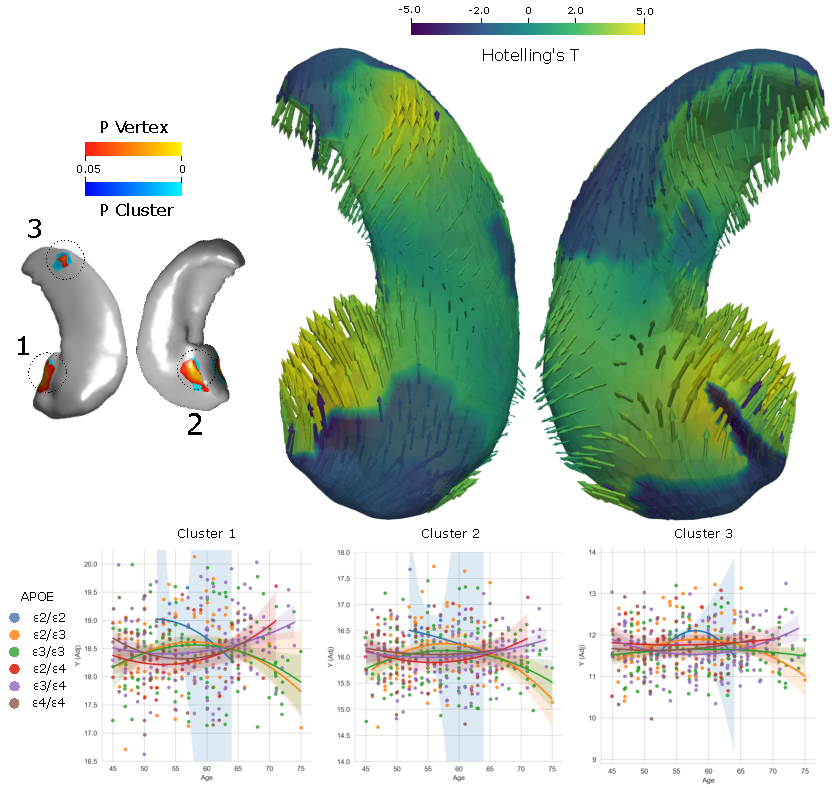
\includegraphics[width=0.9\textwidth]{figures/hippocampus/fig_interactionapoealfa_OR.pdf}
  \caption[Quadratic interaction between APOE OR for AD and age on the right hippocampus.]{Quadratic interaction between APOE OR for AD and age on the right hippocampus after adjusting for other covariates, for all possible allele pairs. Positive values (coloured in light yellow) indicates expansion. Negative values (coloured in dark violet) indicates contraction. Arrow length and size indicate a stronger effect. For the interaction plots, Y(adj) is the magnitude of the adjusted $y$ variable on the detected cluster. Shaded gray areas indicate $90\%$ confidence intervals.}\label{fig:alfainteractionfig2}
\end{figure}

\subsection{ADNI dataset}

For the ADNI cohort, after preprocessing (Section \ref{sec:pipeline}) and discarding subjects with segmentation errors, we ended up with 969 patients. Supplementary Table S6 shows the ID of all ADNI subjects used in the study. \\

Table \ref{table:fullADNItable} summarizes the main results for all the experiments, using the models described in Section \ref{subsec:exp}. "Base model" section shows the effects for age, sex, site, years of education, APOE and DX. Figure \ref{fig:adnibaselinefig1} shows the effects of selected factors on the surface of both hippocampi. Similar to what happened in ALFA, age and sex present a general contraction over the surface. DX and APOE also show a general contraction effect. No significant clusters were found on the effect of acquisition sites. "Interactions" section of Table \ref{table:fullADNItable} shows the results of models with and squared interactions between APOE and age, and between DX and age. For the interaction model between age and diagnosis, no significant clusters were detected. Full results for the interaction model between age and diagnosis and diagnosis and APOE are included in Supplementary Tables S7 and S8. \\

\begin{table}[htbp]
\centering
\resizebox{0.9\textwidth}{!}{%
\begin{tabular}{@{}c|c||ccc||ccc@{}}
\toprule
 & \multirow{2}{*}{Test} & \multicolumn{3}{c||}{Results}  & \multicolumn{3}{c}{Cluster analysis} \\  \cline{3-5} \cline{6-8}
 &  & Hipp & Avg. T & Max. T & N & $P_{peak}$ & $P_{cluster}$ \\ \midrule
\multirow{17}{*}{\rotatebox[origin=c]{90}{Base model}} & Age &    R &  1.76 &   13.45 & 2379 &   $<0.001$ &  $<0.001$  \\
&    &    L &   1.75 &  14.3 & 2185 &    $<0.001$ &  $<0.001$ \\
& Sex    &    R &  2.19 &  12.85 &  2488 &  $<0.001$ & $<0.001$ \\
&       &    L &   2.17 &  13.73 & 2375 &   $<0.001$ & $<0.001$ \\
& Site &    R &    0.64 &   3.60 &  - & - & - \\
&      &    L &   0.65 &   3.24 & - & - & - \\
& Years ed. &    R & 0.80 &   4.33 &  109 &   0.029 &  0.003 \\
&           &    L & 0.73 &   4.06 &  - & - & - \\
& APOE (Add) &   R &    0.9 &  5.1 &  234 & 0.001  & $<0.001$  \\
&                         &   &   &    & 144 & 0.013 &  0.003 \\
&              &    L &   1.02 &   6.38 &   529 &  $<0.001$ &  $<0.001$ \\
&              &     &    & &   304 &  $<0.001$ &  $<0.001$ \\
& APOE ($\log$(OR)) &   R &   0.92 &   5.06 & 476 &  0.002 &  $<0.001$ \\
&           &   L &   1.04 &   6.34 &  1223 &    $<0.001$  &   $<0.001$  \\
& DX (AD>MCI>CN) &   R &   1.65 &  10.10 & 2383 &     $<0.001$  &   $<0.001$  \\
&                &   L &   1.65 &  11.59 &  2289 &  $<0.001$  &  $<0.001$  \\ \midrule
\multirow{14}{*}{\rotatebox[origin=c]{90}{Interactions}} & APOE (Add)$\times$Age &    R & 0.58 &   3.02 & - & - & -  \\ 
&                     &    L &   0.68 &   3.54 & - &  - & - \\ 
& APOE (Dom)$\times$Age &    R &   0.6 &   2.87  &  - & - & - \\ 
&                     &    L &   0.72 &  3.54 & - &  - & - \\
&  APOE (Add)$\times$Age$^2$ &    R &   0.55 &   3.06 &  - & - & - \\ 
&                         &    L &    0.64 &   3.42  &  - & - & - \\ 
& APOE (Dom)$\times$Age$^2$ &    R &   0.56 &   2.91   &  - & - & - \\ 
&                        &    L &    0.65 &   3.51 & - & - & - \\ 
& APOE ($\log$(OR)))$\times$Age$^2$ &    R & 0.54 & 2.74 &  - & - & - \\ 
&                        &    L & 0.6  & 3.29  & - & - & - \\ 
& APOE ($\log$(OR)))$^2\times$DX &  R & 0.65 & 3.17 &  - & - & - \\ 
&                        &    L & 0.7  & 3.94 & - & - & - \\ 
& (AD > MCI) $\times$Age$^2$ &    R &   0.71 &  3.38   &  - & - & - \\ 
&                          &    L &    0.75 &   3.84 & - &  - & - \\  \bottomrule
 \bottomrule
\end{tabular}}
\caption[Results obtained on the ADNI cohort for base, linear interaction, and squared interaction models.]{\small Results obtained on the ADNI cohort for base, linear interaction, and squared interaction models. General test results and information about significant clusters that survived correction are included. Results are divided by model (base, linear interaction or squared interaction). Hipp indicates left (L) or right (R) hippocampus. Max. and Avg. T are the maximum and average Hotelling's T statistic over all vertices, respectively. XX > YY indicates the comparison used for that specific test. For the cluster analysis after correction, N is the number of vertices of the significant cluster. $P_{peak}$ and $P_{cluster}$ are the random field corrected p-values for the peak point and the whole cluster, respectively. Only  clusters with N > 20 and $P_{cluster} < 0.05$ are included. DX: diagnosis. Rec: recessive. Add: additive. Dom: dominant. OR: Odds risk.}\label{table:fullADNItable}
\end{table}

\begin{figure}[htbp]
  \centering
  \includegraphics[width=0.75\textwidth]{figures/hippocampus/baseline_hippo_adni.pdf}
  \caption[Directional effect on the surface of the hippocampus, ADNI cohort.]{Directional effect on the surface of the hippocampus for (from top to bottom) age, sex, site, years of education, APOE and DX. ADNI cohort with the base model. Positive values (colored in light yellow) indicates expansion. Negative values (colored in dark violet) indicates contraction. Arrow length and size indicate a stronger effect.}\label{fig:adnibaselinefig1}
\end{figure}
%htbp

On the comparison between healthy patients, ADNI includes 256 cognitively healthy patients, with a relatively low proportion of $\varepsilon4$-homozygotes (6 patients, less than $5\%$). For this reason, it is difficult to extract meaningful conclusions from the experiments. We tested for main effects and interactions between APOE and age to detect any similarities to the results obtained in ALFA, considering that the obtained results will not have enough statistical power to draw meaningful conclusions. Supplementary file S9 shows the effect on the surface of the hippocampus for APOE and the interaction between age and APOE. \\

\subsection{Similarity between effects}
\label{sec:similarity}
\definecolor{Gray}{gray}{0.9}

We quantitatively assessed the similarity between different effects obtained in our tests. Table \ref{table:sim} shows the results for the different selected comparisons. Comparisons 1 to 4 are designed to study similarities between APOE effects and DX effects, whereas comparisons 5 to 8 are aimed to study similar APOE effects across different cohorts. The most relevant comparisons, due to their relevancy or strong effect detected are highlighted in grey and shown in more detail in Supplementary Figure S10, including the effect maps for both compared effects, the full similarity map, and the significant clusters discovered after the randomization testing (Section \ref{sec:visualization}). Figure \ref{fig:sim_2} shows a comparison between the effects of the square additive interaction between age and APOE in ALFA, and the effect of the negative squared interaction between age and diagnosis in ADNI, and the corresponding discovered clusters, observing strong similarities in several regions of the hippocampus for both comparisons. For further results on the similarity tests, Supplementary Table S11 shows similarities between same effects on different cohorts and Supplementary Files S12 and S13 contains the full results for all conducted tests, for the APOE $\varepsilon$4 load models and AD OR model respectively. \\

\begin{figure}[htbp]
  \centering
  \includegraphics[width=0.9\textwidth]{figures/hippocampus/sim_figure_2.pdf}
  \caption[Effects of the squared additive interaction between age and APOE in ALFA.]{Effects of the squared additive interaction between age and APOE in ALFA dataset (above) and the effects of the negative squared interaction between diagnosis and age in ADNI (below). Both hippocampus are represented.}\label{fig:sim_2}
\end{figure}

\begin{table}[htbp]
\centering
\resizebox{0.95\textwidth}{!}{%
\begin{tabular}{@{}p{7cm}cccccc}
 \toprule
Comparison  & Effect 1 & Effect 2 & Hipp & Sim & N    & P     \\ \midrule
\multirow{10}{*}{1. ALFA base - ADNI base}  & APOE (Add)      & Age      & R    & 0.55 & 55 & 0.028\\
                              &          &          & L    & 0.51 & 72 & 0.028 \\
                              & APOE (Add)      & Years ed.      & R    & 0.61 & 109 & 0.028  \\
                              &          &          & L    & 0.56 & 234  & 0.031 \\
                              & APOE (Add)   & APOE (Add)      & R   & 0.66 & 290 & 0.026  \\ 
                              &              &                 & L   & 0.61 & 173 & 0.036 \\ 
             & \cellcolor{Gray} APOE (Add)      & \cellcolor{Gray} DX  & \cellcolor{Gray} R   & \cellcolor{Gray} 0.62 & \cellcolor{Gray} 268 & \cellcolor{Gray} 0.021 \\ 
           &   \cellcolor{Gray}         &   \cellcolor{Gray}       &  \cellcolor{Gray} L    & \cellcolor{Gray} 0.58 & \cellcolor{Gray} 213 & \cellcolor{Gray} 0.022 \\  
             &  APOE ($\log$(OR))  & APOE ($\log$(OR))  & R   & 0.56  & 79 & 0.022 \\ 
           &       &          & L    & 0.58 & 221 & 0.014 \\  \midrule
%%% 2
\multirow{6}{*}{2. ALFA (linear int.) - ADNI base}  & \cellcolor{Gray} Age$\times$APOE (Add) & \cellcolor{Gray} DX  & \cellcolor{Gray} R    & \cellcolor{Gray} 0.60 & \cellcolor{Gray} 239 & \cellcolor{Gray} 0.025 \\
      &  \cellcolor{Gray}   & \cellcolor{Gray}  & \cellcolor{Gray} L & \cellcolor{Gray} 0.49 & \cellcolor{Gray} 96  & \cellcolor{Gray} 0.020 \\
                               & Age$\times$APOE (Add) & APOE (Add)  & R  & 0.57 & 212 & 0.023 \\
                           &          &          & L    & 0.54 & 92  & 0.022 \\
%                               & AgexAPOE (Add) & Age  & R  & 0.7 & 295 & 0.02  \\
%                           &          &          & L    & 0.49 & 39  & 0.02 \\
       & \cellcolor{Gray} Age$\times$APOE (Dom) & \cellcolor{Gray} APOE (Dom)  & \cellcolor{Gray} R    & \cellcolor{Gray} 0.59 & \cellcolor{Gray} 233 & \cellcolor{Gray} 0.024 \\
     &    \cellcolor{Gray}  & \cellcolor{Gray} & \cellcolor{Gray} L    & \cellcolor{Gray} 0.51 & \cellcolor{Gray} 109  & \cellcolor{Gray} 0.021 \\ \midrule
%%% 2.2
\multirow{8}{*}{3. ALFA (sq int.) - ADNI base} & \cellcolor{Gray} Age$^2$xAPOE (Add) & \cellcolor{Gray} DX  & \cellcolor{Gray} R    & \cellcolor{Gray} 0.50 & \cellcolor{Gray} 154 & \cellcolor{Gray} 0.021 \\
  & \cellcolor{Gray}  & \cellcolor{Gray} & \cellcolor{Gray} L    & \cellcolor{Gray} 0.62 &\cellcolor{Gray} 273  & \cellcolor{Gray} 0.019 \\
                               &  Age$^2$xAPOE ($\log$(OR)) & DX  & R  & 0.60 & 131 & 0.022 \\
                                &         &          & L    & 0.63  & 275 & 0.019 \\
                               & Age$^2\times$APOE (Add) & APOE (Add)  & R    & 0.50 & 187 & 0.023 \\
                               &          &          & L    & 0.58 & 240  & 0.019 \\
                               & Age$^2\times$APOE (Dom) & APOE (Dom)  & R    & 0.50 & 199 & 0.019 \\
                               &          &          & L    & 0.53 & 213  & 0.019 \\ \midrule
%%% 3
\multirow{4}{*}{4. ALFA (sq int.) - ADNI (sq int.)} & \cellcolor{Gray} Age$^2\times$APOE (Add) & \cellcolor{Gray} -Age$^2\times$DX  & \cellcolor{Gray} R    & \cellcolor{Gray} 0.87 & \cellcolor{Gray} 686 & \cellcolor{Gray} 0.022 \\
                  &  \cellcolor{Gray}   &  \cellcolor{Gray} & \cellcolor{Gray} L    & \cellcolor{Gray} 0.81 & \cellcolor{Gray} 274  & \cellcolor{Gray} 0.028 \\ 
&  \cellcolor{Gray} Age$^2\times$APOE ($\log$(OR)) & \cellcolor{Gray} -APOE ($\log$(OR)) $\times$DX  & \cellcolor{Gray} R    & \cellcolor{Gray} 0.68 & \cellcolor{Gray} 218 & \cellcolor{Gray} 0.02 \\
                  & \cellcolor{Gray}  & \cellcolor{Gray}  & \cellcolor{Gray} L    & \cellcolor{Gray} 0.66 & \cellcolor{Gray} 270 & \cellcolor{Gray} 0.02 \\ \midrule
%% 4
\multirow{2}{*}{5. ALFA base - ADNI NC base} & \cellcolor{Gray} APOE (Add)   & \cellcolor{Gray} APOE (Add)  & \cellcolor{Gray} R   & \cellcolor{Gray} 0.70 & \cellcolor{Gray} 169 & \cellcolor{Gray} 0.026  \\ 
                              & \cellcolor{Gray}   & \cellcolor{Gray} &  \cellcolor{Gray} L   & \cellcolor{Gray} 0.61 & \cellcolor{Gray} 201 & \cellcolor{Gray} 0.023 \\ \midrule
\multirow{2}{*}{6. ALFA (sq int.) - ADNI NC (sq int.)} & Age$^2\times$APOE (Dom) & Age$^2\times$APOE (Dom)  & R    & 0.53 & 190 & 0.033 \\
                               &     &          & L    & 0.44 & 35 & 0.021 \\ \midrule
\multirow{4}{*}{7. ALFA base - ALL base}  &  APOE (Add)      & DX   & R   & 0.63 & 260 & 0.021 \\ 
                              &      &          & L    & 0.58 & 206 & 0.024 \\
                              &   APOE (Dom)      & APOE (Dom)   & R   & 0.57 & 155 & 0.030 \\ 
                              &       &          & L    & 0.62 & 135 & 0.036 \\ \midrule
\multirow{2}{*}{8. ALFA (sq int.) - ALL (sq int.)}     & Age$^2\times$APOE (Dom) & Age$^2\times$APOE (Dom)  & R  & 0.34 & - & - \\
                               &          &          & L    & 0.36 & 20 & 0.019 \\ \bottomrule 
\end{tabular}}
\caption[Similarity results between effects.]{\small Similarity results between effects. Hipp indicates left (L) or right (R) hippocampus. Sim is the mean similarity for all vertices. XX > YY indicates the comparison used for that specific test. N is the number of vertices of the significant cluster. P is the mean p-value of the significant cluster. Only the largest detected cluster of each test is included in the table. Only clusters with N > 20 and $P_{cluster} < 0.05$ are included. DX: diagnosis. Add: additive. Dom: dominant. Rows highlighted are shown in more detail in Supplementary Figure S10.}\label{table:sim}
\end{table}

\section{Discussion}
\label{sec:discussion}

%%% 0 introducció.
In this chapter, we investigated the effect of APOE $\varepsilon4$ allele load on the surface of the hippocampus. We used multiple linear regression to single out the effect of covariates over the hippocampal surface and analyzed linear and non-linear interactions between APOE $\varepsilon$4 allele load and age on the hippocampal surface, while taking into account the reduced risk associated with the $\varepsilon$2 allele. We worked with a cohort of cognitively unimpaired subjects with high genetic risk (ALFA). We additionally applied our processing pipeline to a different dataset with subjects at different stages of the disease (ADNI), to study if the interactions and the APOE effect detected in ALFA can be related to the effect of the disease in individuals along the disease continuum. We show some areas of the hippocampus where APOE $\varepsilon$4 effect is comparable to the effect of the disease, suggesting that those regions could be affected similarly by APOE before disease onset. To our knowledge, this is the first study that explores interactions between APOE $\varepsilon4$ and age on the hippocampal surface using a homozygote enriched dataset of healthy subjects and compares the results to a dataset of subjects at various stages of the disease. \\

When adding a linear interaction term to our model for the ALFA dataset between additive APOE effect and age, we detected significant effects (Table \ref{table:fullALFAtable}, linear interaction model) in the CA1 of both hemispheres (Supplementary Figure S3, S4)\footnote{We used the hippocampal subfield map from \cite{Iglesias2015} as reference.}. It is worth noting that this effect, while appearing in a dominant model, is not significant when encoding the AD odds risk model. When adding a squared interaction to the model, APOE OR interactions with age and age squared presented strong effects in the CA1, parasubiculum and GC-DG, and on a zone between CA3, CA1, and HATA of the right hippocampus (Figure \ref{fig:alfainteractionfig2}). When observing the interaction in those zones, we see that they are grouped with respect to APOE $\varepsilon$4 allele load (Figure \ref{fig:alfainteractionfig2}, bottom), although the interaction with $\varepsilon$2$\varepsilon$2 has large uncertainty due to the low number of samples (Table \ref{table:apoeallele}). Those results were also observed when using a simpler additive model, although the smallest cluster was not detected (Supplementary Figure S5). Those areas were also detected when comparing HE to NC. However, dominant and recessive models did not detect significant clusters in those areas. \\

Findings agree with previous studies on the effect of APOE on hippocampus volume \cite{Pievani2011,Mueller2009,Cacciaglia2018}, where strong interactions between APOE $\varepsilon$4 allele load and hippocampal volume in cognitively unimpaired subjects were detected. Going beyond those results, we have been able to suggest specific areas where that interaction is stronger, suggesting that how age affects hippocampal morphology depends strongly on the APOE allele, something that has also been detected by other researchers \cite{Shi2014}. Such effects can be interpreted as if the interaction between APOE and age is different between hippocampi: there is a linear interaction in both hippocampus, and in the right hippocampus, APOE and age present significant interactions that have less impact at a higher age. Regarding the protective effect of $\varepsilon$2, we could not observe a significant effect on our experiments, given the similarity of the interaction with pairs with and without $\varepsilon$2 and the uncertainty due to the low amount of $\varepsilon$2$\varepsilon$2 samples (Figure \ref{fig:alfainteractionfig2}, bottom). \\

Without introducing interactions in ALFA, APOE does not seem to capture large variations in shape, and indeed, no clusters survived correction (Table \ref{table:fullALFAtable}), in any of the tested APOE models. Subtle differences between APOE groups cannot be easily detected on surface-based studies of the hippocampus, something also observed in other studies with a different cohort of patients \cite{Dong2019}, where such differences were subtle, even before correction. Age presented large effects over the whole surface, being most of them significant after correction, as shown in Table \ref{table:fullALFAtable} and Figure \ref{fig:alfabaselinefig1}, an expected result given that age is a known factor affecting hippocampus shape and volume \cite{Lind2006}, and the association between sex and intracranial volume. \\ 

Our tests in the ADNI dataset show that the pipeline and the analysis methods are able to capture changes and deformations that agree with current knowledge of the effect that AD has on the hippocampus (Table \ref{table:fullADNItable}). We observed that age, sex, years of education, and site present significant differences after correction in large regions of the bilateral hippocampi. Differences between AD stages were also strong, showing a general contraction over all the surface of the hippocampus (Figure \ref{fig:adnibaselinefig1}), showing the atrophy caused by the disease. APOE effect also presented a general atrophy effect over the surface, similar to the AD effect. This similarity can be explained by the unequal distribution of patients for each diagnosis (Table \ref{table:cohorts}), with demented patients having higher APOE based risk. We did not find any significant interactions between APOE $\varepsilon$4 and age in ADNI (Table \ref{table:fullADNItable}). We did find an interaction between APOE $\varepsilon$4 and DX on the left hippocampus between AD and MCI groups (Table \ref{table:fullADNItable}), but no other significant results with any other contrasts (Supplementary Table S8), which suggests that APOE $\varepsilon$4 impacts the three tested stages of AD in a similar way, with a small interaction between MCI and AD. We also tested for interaction between APOE OR and AD diagnosis to see if a protective effect of $\varepsilon$2 could appear, but no significant interactions were found. \\

Apart from the already mentioned findings on age and APOE interaction on ALFA dataset, we have not detected large differences between our different model encodings of the allele information. Recessive and dominant models did not reveal further zones or interactions that were not already detected by the other models, and additive models (Supplementary Figure S5) and AD OR models (Figure \ref{fig:alfainteractionfig2}) were the most informative models. Effect maps and results were also very similar between models (Table \ref{table:fullALFAtable}, Figure \ref{fig:alfabaselinefig1}). This indicates that the effect of APOE $\varepsilon$4 allele load could be modelled more appropriately in a linear (additive) way, or encoding empirical knowledge of the risk to the model \cite{Reiman2020}. \\

We studied the similarities between APOE $\varepsilon$4 effects and DX effects over ALFA and ADNI cohorts. Results between the same effects (e.g. age vs age, sex vs sex) on different cohorts (shown in Supplementary Table S10) show high similarity, showing that the results are comparable between cohorts. Table \ref{table:sim} (comparisons 1-4) show that, for baseline effects, there are some areas in the tail and presubiculum of the hippocampus where a high similarity can be found, with significant clusters detected in the right hippocampus. This could indicate that even if in our previous tests those regions did not have a strong enough statistical power, APOE $\varepsilon$4 could affect those regions before the onset of the disease, and leave them more vulnerable to the atrophy caused by AD, which is consistent with existing literature on this relationship \cite{Wolk2010}. However, as previously mentioned, AD and APOE $\varepsilon$4 effects on ADNI (observed in Figure \ref{fig:adnibaselinefig1}) have a general atrophy effect over the surface, so the found significant areas could simply be regions where APOE produces a contraction effect. We found a large similarity in the interaction effect between squared age and APOE in the ALFA dataset and the inverse interaction effect between squared age and diagnosis in ADNI, with several large significant clusters. This result suggests that age modulates the effect of both APOE and DX over a specific local area on the hippocampal surface similarly, being a direct effect for APOE and an inverse effect for DX. Figure \ref{fig:sim_2} shows a larger version of both effect maps, where the similarities between effects can be better appreciated. The similarity is especially high in the right hippocampus, where the interaction between APOE and age in CN subjects is significant (Figure \ref{fig:alfainteractionfig2}). Comparing the similarities obtained using the APOE odds risk model, they are very similar to the ones obtained using additive/dominant models, in line with previous observations (Supplementary Tables 12 and 13).  \\ 

We tested our method on a subset of the ADNI dataset to be able to directly compare two different cohorts of cognitively healthy patients, and we also did additional analysis by combining both cohorts. Table \ref{table:sim} (comparisons 5 to 8) shows the obtained results. We compared between APOE effects, between APOE and DX effects, and between interactions. Similar areas were found, but the detected significant clusters are small and non-conclusive. For the combination of cohorts, no significant results were found (Supplementary Tables S1 and S2, and Supplementary Figures S14 and S15). This lack of significant results could suggest that the interaction effect detected in ALFA is strongly influenced by the $\varepsilon4$ homozygotes, of which the ADNI cohort has a lower proportion. \\ 

We conjecture three (non-exclusive) reasons for the results obtained in those comparisons. First, the site variable for the combined cohort (we added a new category for ALFA subjects) captured much more variation than in previous tests with only ADNI patients, where differences were not significant. This variation shows that differences in image acquisition and protocols between sites greatly influence the MRI scan and hence the corresponding hippocampus mesh. Second, the age disparity between datasets (Supplementary Figure S16). ADNI individuals are older than ALFA ones, due to differences in study recruitment and aim (ALFA focuses on cognitively healthy subjects, with no signs of disease, whereas ADNI focuses on subjects that are already in the AD continuum). This difference in age distribution could also explain why the detected interactions in ALFA are not present in ADNI, should such interactions only happen (or be more apparent) at an earlier age. Finally, there could exist other population differences that are not being accounted for. \\

Our study presents various limitations. First, even if our analysis allows for testing any effect on the surface of the hippocampus, we focused on APOE $\varepsilon$4 allele load and interactions with age. We could add to our analysis other risk factors, such as relevant genotypic factors, cognitive scores, or lifestyle and cardiovascular factors. One key advantage of ADNI over ALFA at this stage is the availability of biomarker status on cerebrospinal fluid. $A\beta$ levels in ADNI could be used to disentangle whether differences observed in ALFA might be due to abnormal amyloid levels or interactions with such levels. However, previous reports have determined that the impact of amyloid accumulation on morphological changes in the brain of cognitively unimpaired individuals is low, as well as any interactive effects of APOE $\varepsilon$4 \cite{Liu2015c,Lim2017}. For multimodal analysis, methods such as multiple kernel learning, which has been used on other types of medical data for disease characterization, could be used \cite{Sanchez-Martinez2017,Marti-Juan2019}. Another interesting line of work is to directly study the deformations and effects that happen at different hippocampus subfields, similar to Zhao et al.\ \cite{Zhao2019}. Second, our analysis were limited to the hippocampus region, but we could extend them to other parts of the brain that present differences in healthy subjects, such as the ventricles. Third, given the large effect of the site in our analysis, segmentation should be improved to ensure robust comparisons between datasets. Moreover, we only used cross-sectional data. Extending our analysis to a longitudinal cohort may allow us to test the shape changes over time, which could also be affected by APOE $\varepsilon$4. \\

\section{Conclusions}
\label{sec:conclusions}

In this article, we have studied differences in hippocampal surface shape on a cohort of genetically enriched cognitively healthy subjects. We have shown a linear and quadratic interaction between APOE $\varepsilon$4 allele load and age on two different surface regions of the right hippocampus. We have also applied the same method to a different cohort of subjects (including both cognitively impaired and unimpaired subjects) and detected remarkable similarities between the APOE interaction with age in asymptomatics and the effect of the disease in a second cohort. Results suggest that for late/middle-aged cognitively unimpaired subjects, APOE $\varepsilon$4 exerts an effect on the hippocampal surface comparable to that observed in clinical stages of AD but to a lower extent. In addition, these effects interacted with age, showing a remarkable similarity across the two studied cohorts. \\

\section*{Acknowledgements}
This publication is part of the ALFA study (ALzheimer and FAmilies). The authors would like to express their most sincere gratitude to the ALFA project participants, without whom this research would have not been possible. The project leading to these results has received funding from “la Caixa” Foundation (ID 100010434), under agreement LCF/PR/ GN17/50300004. Additional support has been received from the Universities and Research Secretariat, Ministry of Business and Knowledge of the Catalan Government under the grant no. 2017-SGR-892. This work was also partially funded by the Spanish Ministry of Economy and Competitiveness under the María de Maeztu Units of Excellence Programme 525 [MDM-2015-0502]. JDG is supported by the Spanish Ministry of Science, Innovation and Universities - State Research Agency (RYC-2013-13054). \\

Data collection and sharing for this project was funded by the Alzheimer's Disease Neuroimaging Initiative (ADNI) (National Institutes of Health Grant U01 AG024904) and DOD ADNI (Department of Defense award number W81XWH-12-2-0012). ADNI is funded by the National Institute on Aging, the National Institute of Biomedical Imaging and Bioengineering, and through generous contributions from the following: AbbVie, Alzheimer’s Association; Alzheimer’s Drug Discovery Foundation; Araclon Biotech; BioClinica, Inc.; Biogen; Bristol-Myers Squibb Company; CereSpir, Inc.; Cogstate; Eisai Inc.; Elan Pharmaceuticals, Inc.; Eli Lilly and Company; EuroImmun; F. Hoffmann-La Roche Ltd and its affiliated company Genentech, Inc.; Fujirebio; GE Healthcare; IXICO Ltd.; Janssen Alzheimer Immunotherapy Research {\&} Development, LLC.; Johnson {\&} Johnson Pharmaceutical Research {\&} Development LLC.; Lumosity; Lundbeck; Merck {\&} Co., Inc.; Meso Scale Diagnostics, LLC.; NeuroRx Research; Neurotrack Technologies; Novartis Pharmaceuticals Corporation; Pfizer Inc.; Piramal Imaging; Servier; Takeda Pharmaceutical Company; and Transition Therapeutics. The Canadian Institutes of Health Research is providing funds to support ADNI clinical sites in Canada. Private sector contributions are facilitated by the Foundation for the National Institutes of Health (\url{www.fnih.org}). The grantee organization is the Northern California Institute for Research and Education, and the study is coordinated by the Alzheimer’s Therapeutic Research Institute at the University of Southern California. ADNI data are disseminated by the Laboratory for Neuro Imaging at the University of Southern California. Data used in preparation of this article were obtained from the Alzheimer’s Disease Neuroimaging Initiative (ADNI) database. As such, the investigators within the ADNI contributed to the design and implementation of ADNI and/or provided data but did not participate in analysis or writing of this report. A complete listing of ADNI investigators can be found at\footnote{\url{http://adni.loni.usc.edu/wp-content/uploads/how_to_apply/ADNI_Acknowledgement_List.pdf}}. \\

Collaborators of the ALFA study are: Eider M. Arenaza-Urquijo, Alba Cañas, Carme Deulofeu, Ruth Dominguez, Karine Fauria, Marta Félez-Sánchez, José M. González de Echevarri, Xavi Gotsens, Oriol Grau-Rivera, Laura Hernandez, Gema Huesa, Jordi Huguet, Paula Marne, Tania Menchón, Marta Milà-Alomà, Carolina Minguillon, Maria Pascual, Albina Polo, Gonzalo Sánchez-Benavides, Sandra Pradas, Aleix Sala-Vila, Anna Soteras, Marc Suárez-Calvet, Laia Tenas, Marc Vilanova, Natalia Vilor-Tejedor. \\

Parts of the data that support the findings of this study are available from Alzheimer’s Disease Neuroimaging Initiative (ADNI). Restrictions apply to the availability of these data, which were used under license for this study. Data are available at http://adni.loni.usc.edu/ upon application. ALFA study data that support the findings of this study are available from the corresponding author upon reasonable request. 

